%!TEX root=../../main.tex
\section{Datenschnittstelle zwischen Frontend und Backend und Webseitenlogik}
Die Schnittstelle zwischen Frontend und Backend soll mittels eines JavaScript-Frameworks umgesetzt werden. Der Studie nach, wird hierfür VueJS verwendet. VueJS bietet viele passende Funktionen und Features um solch eine Webseite umzusetzen.
\subsection{Webseitenlogik}
Die Webseite soll mittels Vue-Komponenten aufgebaut werden. Eine Seite besteht aus einer Hauptkomponente und möglicherweise noch zusätzliche Nebenkomponenten. Die Struktur der einzelnen Komponenten und Links der Webseite soll wie folgt aussehen:
\begin{figure}[H]
	\centering
	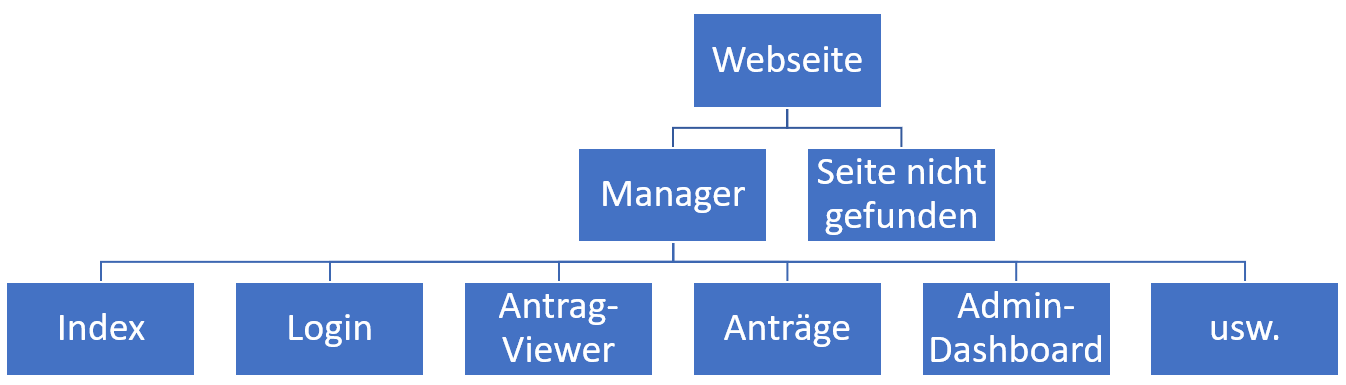
\includegraphics[width=0.8\linewidth]{images/Webseite_hierarchie}
	\caption[Die Hierarchie der Webseite]{Die Übersicht der Hierarchie der Webseite.}
	\label{fig:webseitehierachie}
\end{figure}

\subsubsection{Seite wurde nicht gefunden}
Sollte ein Link eingegeben werden, welcher nicht die Seite selbst, oder eine definierte Unterseite ist, soll eine Seite geladen werden, bei der der Benutzer darauf hingewiesen wird, dass er keinen korrekten Link eingegeben hat.
\subsubsection{Manager}
Der Manager soll der Hauptbestandteil der Webseite sein. Er wird alle einzelnen Seiten beinhalten und immer die gewünschten Seiten anzeigen. In dem Manager werden auch Cookie-Einstellungen und Rechte gespeichert. Fast alle Komponenten sollen dem Manager untergeordnet sein. Der Manager soll auch dafür verantwortlich sein zwischen Komponenten Daten zu senden.

\subsubsection{Navigation}
Da fast alle Komponenten dem Manager untergeordnet ist, ist es auch die Verantwortung des Managers die Navigation zu steuern. Dazu soll es eine zentrale Funktion im Manager geben, welche die derzeit geladene Seite verändern kann. Des Weiteren sollen die benötigten Informationen geladen bzw. erstellt werden, welche die Komponenten benötigen.
\\\\
Die Funktion zum Verändern der derzeitigen Anzeige, soll von den untergeordneten Komponenten aufgerufen werden. Hinzu kommt, dass mit dem Aufruf der Funktion auch spezifiziert werden soll, welche Seite geladen werden muss. Falls spezielle Seiten geladen werden, sollen die zusätzlichen Informationen über diese Funktion mitgegeben werden.

\subsubsection{Komponenten}
Einzelne Komponenten sollen die Daten eigenständig aus dem Backend laden. Nur im Falle, dass eine Komponente Daten an eine Weitere sendet, soll dies über den Manager geschehen. In den jeweiligen Komponenten soll auch jeder Befehl eigenständig an das Backend gesendet werden. Dies sind Maßnahmen, um den Manager nicht mit Funktionen zu überladen und damit keine Daten bei jedem Aufruf von dem Manager an die einzelnen Komponenten gesendet werden müssen.

\subsubsection{Antrag-Viewer}
Es soll eine weitere Komponente vorhanden sein, auf der man durch einen Link gelangen kann. Auf dieser Seite soll es möglich sein, einen Antrag per z.B: ID anzeigen zu lassen. Dieser extra Link, soll nahtlos dem Manager untergeordnet sein. Der Antrag-Viewer soll nur verwendbar sein, sofern der Benutzer angemeldet ist und auch die Berechtigung hat, diesen Antrag anzuschauen.
\\\\
Sollte in dem Link bereits spezifiziert sein, welcher Antrag geöffnet werden soll, kann nach der Anmeldung der Benutzer diesen Antrag betrachten. Sollte der Benutzer keine Berechtigungen besitzen diesen Antrag zu betrachten, wird eine Fehlermeldung ausgegeben.

\subsubsection{Features}
Es sollen auch Funktionen implementiert werden, welche das Benützen der Webseite erleichtern:
\\\\
Es soll möglich sein, bei erneutem Laden der Webseite auf die zuletzt geöffnete Seite zu gelangen. Auch bei Beenden des Browsers soll sich die Webseite merken, auf welcher Seite der Benutzer gewesen ist und diese bei erneutem Aufrufen der Webseite diese laden.
\\\\
Es soll möglich sein, zwischen den Seiten durch die Browser-Pfeile zu navigieren. Dies ist wichtig, da durch versehentliches Drücken einer falschen Komponente ein Benutzer möglichst schnell wieder auf die vorherige Seite gelangen können muss. Durch die Implementierung der Browser-Pfeile kennt sich der Benutzer bereits aus und kann intuitiv auf die vorherige Seite wechseln.
\newpage
\subsection{Daten aus dem Backend laden}
Auf den Seiten, bei denen es benötigt wird, soll über Funktionen des Frameworks dynamisch Komponenten erstellt und geladen werden. Der Prozess, um Daten aus dem Backend zu laden wird in folgender Grafik beschrieben:
\begin{figure}[H]
	\centering
	
\includegraphics[width=0.8\linewidth]{images/Prozess_Daten_laden}
	\caption[Prozess der Daten zur Anzeige]{Übersicht über den Prozess, welcher Daten aus dem Backend lädt.}
	\label{fig:prozessdatenladen}
\end{figure}

\subsubsection{Webseite wird aufgerufen}
Die Webseite wird aufgerufen und der Benutzer landet auf der Startseite.

\subsubsection{Daten werden geladen}
Auf der Startseite der Webseite sollen die neuesten Nachrichten angezeigt werden, welche für den Lehrer relevant sind. Hierfür müssen aus dem Backend Daten geladen werden. Dies soll über eine Abfrage erfolgen, welche aus dem Frontend gesendet wird.

\subsubsection{Komponenten werden erstellen}
Die geladenen Daten aus dem Backend, sollen mittels Einbindung der Variablen in einzelne Komponenten eingebunden werden.\\
Seiten, auf denen viele gleiche Komponenten sind, werden mittels Schleifen erstellt. Diese sorgen dafür, dass nicht zu viele Komponenten auf der Seite geladen sind, wenn diese nicht gebraucht werden.

\subsubsection{Komponenten werden angezeigt}
Die bereits erstellten Komponenten sollen über die Einbindung in der Webseite angezeigt werden. Dies kann durch einfache Implementierung bei einzelnen Komponenten sein.\\
Komponenten, bei denen viele Gleiche erstellt werden, sollen über eine Schleife alle hintereinander gereiht und angezeigt werden.
Bei den Nachrichten kann man sich jede Nachricht als eine Komponente vorstellen, welche jeweils erstellt und danach angezeigt werden soll.
\newpage
\subsection{Befehle an das Backend senden}
Die Webseite besitzt auch einige Aktionen, die von Benutzern ausgeführt werden können. Diese müssen je nach Aktion eine neue Seite aufrufen, oder einen Befehl an das Backend senden.

\begin{figure}[H]
	\centering
	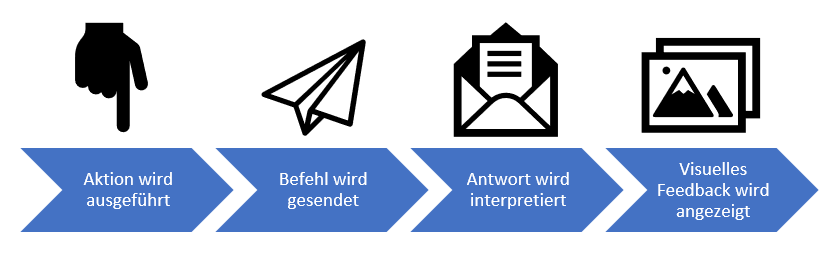
\includegraphics[width=0.8\linewidth]{images/Prozess_Befehl_senden}
	\caption[Prozess der Befehlssendung]{Übersicht über den Prozess welcher Befehle an das Backend sendet.}
	\label{fig:prozessbefehlsenden}
\end{figure}

\subsubsection{Aktion wird ausgeführt}
Eine Aktion wird ausgeführt, wenn z.B: auf eine Komponente gedrückt wird. Dies soll eine Funktion aufrufen, bei der ein Befehl erstellt wird.

\subsubsection{Befehl wird gesendet}
Der Befehl soll alle wichtigen Informationen für das Backend beinhaltet. Beispielsweise, wenn eine neue Nachricht gelöscht werden soll, dann wird die ID der Nachricht mitgesendet.

\subsubsection{Antwort wird interpretiert}
Sobald das Backend den Befehl ausgeführt hat, wird eine Antwort an das Frontend gesendet und soll dort interpretiert werden.

\subsubsection{Visuelles Feedback wird angezeigt}
Sollte ein Fehler aufgetreten sein, soll dem Benutzer dies offensichtlich mitgeteilt werden.\\
Sollte kein Fehler aufgetreten sein, soll dem Benutzer je nach Befehl dies auf unterschiedliche Weise mitgeteilt werden.\\
Um weiterhin das Beispiel zu nutzen: Wenn eine Nachricht gelöscht werden soll, dann wird dem Benutzer mitgeteilt, dass die Nachricht gelöscht worden ist, wenn diese Nachricht verschwindet.